\section{Laboratorio de Active Directory}

En la siguiente sección se van a establecer las directrices para la creación de un laboratorio local que permita la realización de los ataques que se describirán y expemirentación en los capítulos previos a este. La organización de este capítulo es la siguiente: En primer lugar se detallan los requisitos o prerrequisitos necesarios para poder realizar las siguientes acciones como puede ser el software de virtualización, las imágenes del sistema operativo, etc. Posteriormenente, se ha definido y configurado la topología elegida y por último la instalación y administración de Active Directory. 

\subsection{Requisitos}

Previamente a la creación de la topología de red y a la instalción de  Active Directory que permita realizar las pruebas es necesario disponer de las siguientes características.

\subsubsection{Software de virtualización}

La virtualización consiste en la creación de entornos simulados o recursos desde un único sistema operativo denominado {\it host}, por consecuencia, un software de virtualización es aquel que te permite realizar las acciones descritas anteriormente que puede ser la creación de sistemas operativos, creación de topologías de red, administración de recursos etc. Aunque hay gran variadad de sotfware de virtualización, para la realización de este proyecto se ha utilizado {\it Oracle VM VirtualBox}~\cite{Capitulo4:VirtualBox}.\\

{\it VirtualBox} es un software de virtualización {\it Open Source} con licencia GPLv2 desarrollado por Oracle Corporation que permite la creación de entornos x86 and AMD64/Intel64. Para este proyecto se ha utilizado la última versión (VirtualBox 6.0.12) que se puede desacargar en \footnote{https://www.virtualbox.org/}. Con este Software se van a crear las máquinas virtuales y las redes internas necesarias para la creación del laboratorio. 

\subsubsection{Máquinas Virtuales}

Para este proyecto se van a utilizar cuatro máquinas virtuales. Para aquellas que se necesite una licencia de software privativo se va a utilizar la versión de prueba que proporciona Microsoft con el objetivo de que cualquier pueda replicar dicho laboratorio sin necesidad de lincencias adicionales. Las máquinas son las siguientes:

\begin{itemize}
\item \textbf{DC01}: El la máquina virtual principal y es la encargada de administrar el Active Directory. Como se ha comentado en el estado del arte se va a utilizar Windows Server 2019 es su última versión. La imagen del sistema operativo se ha descargado de \footnote{https://www.microsoft.com/en-us/evalcenter/evaluate-windows-server-2019}.

\item \textbf{Cliente01}: Por otro lado, esta máquina representa a la de un usuario legítimo o cliente de una empresa que está unido al dominio y conectado por la red interna. Para esta máquina virtual se ha utilizado Windows 10 Enterprise que se puede descargar en \footnote{https://www.microsoft.com/en-us/evalcenter/evaluate-windows-server-2019}. 

\item \textbf{Gateway}: Esta máquina virtual se va a utilizar como puerta de enlace entre la red interna y la red externa lo que simula ser internet. Para su implementación, se ha utilizado Debian 10 (Buster) sin escritorio para ahorrar recursos locales. La imagen de este sistema operativo se puede descargar en \footnote{https://cdimage.debian.org/debian-cd/current/amd64/iso-cd/debian-10.1.0-amd64-netinst.iso}.

\item \textbf{Atacante01}: Por último, para la simulación de un atacante externo o profesional de la seguirdad ofensiva realizando labores de {\it Red Team}, se ha utilizado la distribución Kali Linux 2019.3, este distribución ofrece gran variedad de herramientas destinadas a la auditoría informática que serán de utilidad a la hora de realizar los ataques propuestos. Para descargar esta distribución se puede a través de \footnote{https://cdimage.kali.org/kali-2019.3/kali-linux-2019.3-amd64.iso}.

\end{itemize}


\subsubsection{Instalación y actualización}

La instalación y actualización de las máquinas, no entra del alcance de este proyecto, por lo tanto, ha quedado reflajado en los Anexos de la literatura.A partir de este punto se da por hecho de que el usuario ha instalado y actualizado las máquinas y cuenta con la última versión de las mismas. 

\subsection{Configuración previa}

Antes de configurar el active directory, se ha creado una topología en red simula a un entorno coorporativo fictio. Aunque este laboratorio únicamente disponga de una máquina unida al dominio, en entornos reales son multitud los equipos lo que posibilita un gran abanico de posibles entradas a la red de la empresa u organización. A contanuación se va a explicar la topología elegida y las configuraciones necesarias.. 

\subsubsection{Topología de red}

Como ya se ha adalentado, la máquina consta de 4 máquinas: 2 Windows (DC01 y Cliente01) y 2 Linux (Atacante01 y Gateway). La distribución de la topología en red se puede observar en la Figura \ref{Topología}. En la imagen se puede apreciar la existencia de dos redes: ADNET(192.168.0.0/24) formada por los dos dos Sistemas Windows que forman parte del dominio de la empresa fictia y EXTNET(10.10.10.0) que emula en una red interna lo que sería estar expuesto a internet en un entorno real. Ambas redes están enlazadas por el Gateway. 

\begin{figure}[t!] %[ht!] para here [b] para bottom [t] para top
\begin{center}
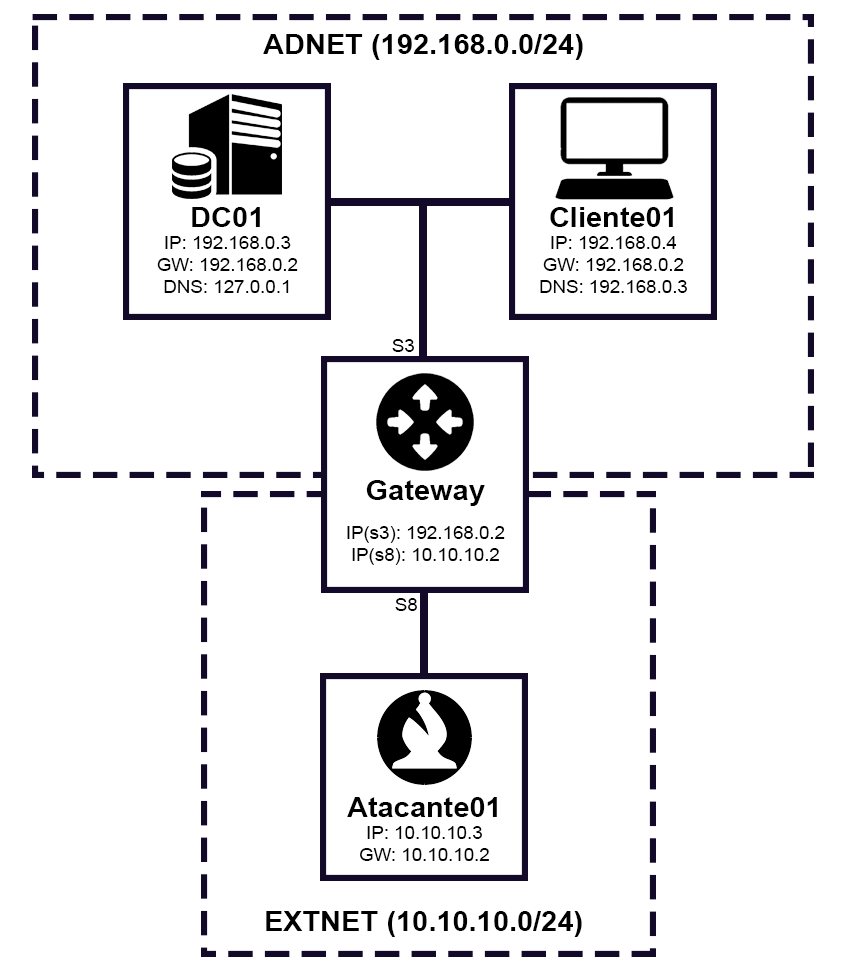
\includegraphics[width=16cm]{Topologia.png}
\end{center}
\caption{Topología del laboratorio local.}
\label{Topología}
\end{figure}

\subsubsection{Configuración de red}

Se va a realizar la configuración necesaria para cada red. 

\begin{itemize}
\item \textbf{DC01}
\begin{enumerate}
\item Antes de arrancar la máquina virtual, es necesario ir a Configuración/Red y añadir el Adaptador1. Esto va a simular la tarjeta de red del DC01. Esta tarjeta de red la vamos a conectar a la red ADNET como se puede ver en la Figura \ref{DC01-Red1}.

\begin{figure}[H] %[ht!] para here [b] para bottom [t] para top
\begin{center}
\includegraphics[width=16cm]{DC01/Red1.png}
\end{center}
\caption{Configuración de red DC01 - Tarjeta de red.}
\label{DC01-Red1}
\end{figure}

\item Una vez iniciada la máquina es necesario dirigirse a {\it Control Panel - Network and Internet - Network Connections} (Figura \ref{DC01-Red2}) y aparecerá la tarjeta de red añadida en el paso anterior. Para editar las direcciones es necesario entrar a las propiedades.
\begin{figure}[H] %[ht!] para here [b] para bottom [t] para top
\begin{center}
\includegraphics[width=16cm]{DC01/Red2.png}
\end{center}
\caption{Configuración de red DC01 - Ajustes de Ethernet.}
\label{DC01-Red2}
\end{figure}

\item Por último, como se puede observar en la Figura \ref{DC01-Red3}, se elige {\it Internet Version Protocol 4(TCP/IPv4) } y después las propiedades de este. Por último, se configura la dirección IP (192.168.0.3), la puerta de enlace correspondiente al Gateway (192.168.0.2) y el DNS. En la mayoría de entornos corporativos es el propio Active Directory el que hace la función de servidor DNS, por lo tanto se escribe la dirección de {\it loopback}: 127.0.0.1.
\begin{figure}[H] %[ht!] para here [b] para bottom [t] para top
\begin{center}
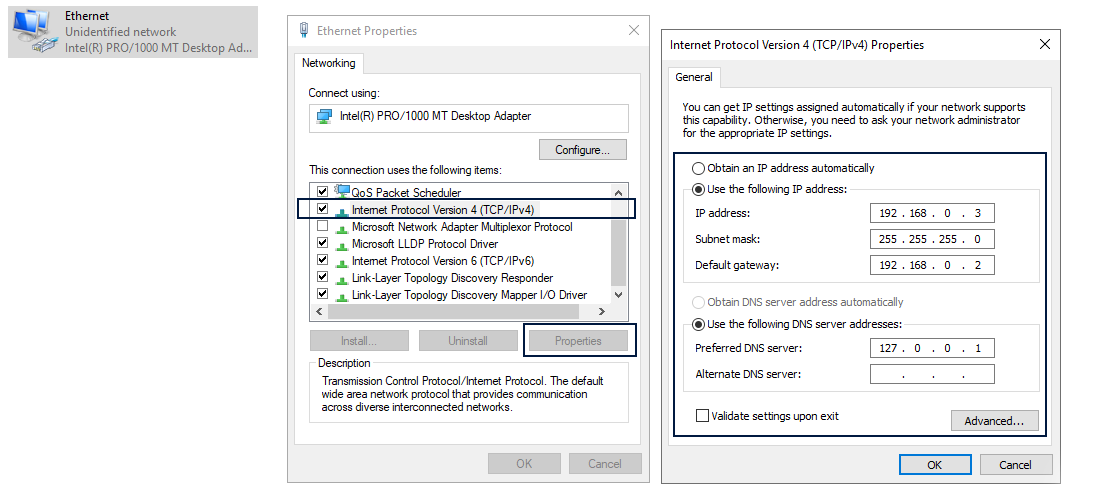
\includegraphics[width=16cm]{DC01/Red3.png}
\end{center}
\caption{Configuración de red DC01 - IPv4.}
\label{DC01-Red3}
\end{figure}
\end{enumerate}

\item \textbf{Cliente01}:
\begin{enumerate}
\item Para configurar la red en el Cliente01, al ser una Máquina Windows en la misma red que el DC01, es necesario repetir los mismos pasos que en la configuración anterior.
\item En el último paso, las direcciones IP son las siguientes: IP(192.168.04) y Gateway(192.168.0.2). En este caso la dirección DNS corresponde a la dirección IP del DC01: 192.168.0.3. La configuración resultante se puede ver en la Figura \ref{Cliente01-Red1}.

\begin{figure}[H] %[ht!] para here [b] para bottom [t] para top
\begin{center}
\includegraphics[width=10cm]{Cliente01/Red1.png}
\end{center}
\caption{Configuración de red Cliente01 - IPv4.}
\label{Cliente01-Red1}
\end{figure}
\end{enumerate}

\item \textbf{Gateway}:

\begin{enumerate}
\item Para esta máquina, es necesario habilitar dos interfaces, una que corresponde a la ADNET o red interna y otra que corresponde con la EXTNET o red externa (Figura \ref{Gateway-Red1}).
\begin{figure}[H] %[ht!] para here [b] para bottom [t] para top
\begin{center}
\includegraphics[width=10cm]{Gateway/Red1.png}
\end{center}
\caption{Configuración de red Gateway - Tarjetas de red.}
\label{Gateway-Red1}
\end{figure}

\item Iniciamos la máquina y comprobamos que se han creado ambas interfaces {\it enp0s3} para la ADNET y {\it enp0s8} para la EXTNET. 

\item A continuación introducimos los siguientes comandos, estos comandos levantan ambas interfaces y asignan las direcciones IP correspondientes. 
\begin{listing}[style=consola, numbers=none]
# ip link set enp0s3 up
# ip a add 192.168.0.2/24 dev enp0s3
# ip link set enp0s8 up
# ip a add 10.10.10.2/24 dev enp0s8
\end{listing}

\item Por último, permitimos que el gateway reenvíe los paquetes que le llegan, para eso se utiliza el siguiente comando: 
\begin{listing}[style=consola, numbers=none]
# echo 1 > /proc/sys/net/ipv4/ip_forward
\end{listing}

\item La configuración final de la máquina se puede observar en la Figura \ref{Gateway-Red2}.
\begin{figure}[H] %[ht!] para here [b] para bottom [t] para top
\begin{center}
\includegraphics[width=15cm]{Gateway/Red2.png}
\end{center}
\caption{Configuración de red Gateway}
\label{Gateway-Red2}
\end{figure}
\end{enumerate}

\item \textbf{Atacante01}:

\begin{enumerate}

\item Esta máquina está en la red externa, por lo tanto añadimos un adaptador de red unida a la red externa (Figura \ref{Atacante01-Red1}). 
\begin{figure}[H] %[ht!] para here [b] para bottom [t] para top
\begin{center}
\includegraphics[width=10cm]{Atacante01/Red1.png}
\end{center}
\caption{Configuración de red Atacante01 - Tarjeta de red}
\label{Atacante01-Red1}
\end{figure}

\item De la misma manera que en el gateway configuramos la interfaz de red, que en este caso es {\it eth0} con los siguientes comandos. 
\begin{listing}[style=consola, numbers=none]
# ip link set eth0 up
# ip a add 10.10.10.3 dev eth0 
\end{listing}

\item Para poder alcazar la red interna, es necesario definir a la dirección 10.10.10.2 como fateway, para que cuando la máquina no encuentre una dirección IP la redirija por ese Gateway. Para ello, se utiliza el siguiente comando: 

\begin{listing}[style=consola, numbers=none]
# ip route default via 10.10.10.2
\end{listing}

\end{enumerate}
\end{itemize}

\subsubsection{Comprobación de la conectividad}

\begin{itemize}

\item \textbf{Cliente01 - DC01}: Para comprobar la conectividad entre Cliente01 y DC10, podemos realizar un ping desde Cliente01 a la dirección IP de DC01 (\ref{Cliente01-Red2}).
\begin{figure}[H] %[ht!] para here [b] para bottom [t] para top
\begin{center}
\includegraphics[width=10cm]{Cliente01/Red2.png}
\end{center}
\caption{Conexión entre Cliente01 y DC01}
\label{Cliente01-Red2}
\end{figure}

\item \textbf{Atacante01 - DC01}: Para comprobar la conectividad dentre Atacante01 y DC10, en vez de realizar un ping intentamos conectarnos a través de Samba (\ref{Atacante01-Red2})
\begin{figure}[H] %[ht!] para here [b] para bottom [t] para top
\begin{center}
\includegraphics[width=10cm]{Atacante01/Red2.png}
\end{center}
\caption{Conexión entre Atacante01 y DC01}
\label{Atacante01-Red2}
\end{figure}

\end{itemize}

\subsubsection{Cambio de nombre del sistema}

Una buena práctica es cambiar el nombre a los Sistemas Windows, esto nos facilitará su identificación y su futura administración. 

\begin{itemize}
\item Para cambiar el nombre a DC01, se puede realizar desde el propio panel de administración del servidor, a través de la opción {\it Local Name Server - Computer Name - Change} como se puede ver en la Figura \ref{DC01-Name1}
\begin{figure}[H] %[ht!] para here [b] para bottom [t] para top
\begin{center}
\includegraphics[width=15cm]{DC01/Name1.png}
\end{center}
\caption{Cambio de nombre DC01}
\label{DC01-Name1}
\end{figure}

\item Para cambiar el nombre a Cliente01, se realiza a través de {\it Control Panel - System and Security - System} posteriormente se elige la opción {\it Change Settings - Change} y se introduce el nombre Cliente01 (\ref{Cliente01-Name1}). Ambos cambios nos van a pedir un reinicio del equipo.  
\begin{figure}[H] %[ht!] para here [b] para bottom [t] para top
\begin{center}
\includegraphics[width=15cm]{Cliente01/Name1.png}
\end{center}
\caption{Cambio de nombre Cliente01}
\label{Cliente01-Name1}
\end{figure}

\end{itemize}

\subsection{Creación y configuración del Active Directory}

\begin{figure}[H] %[ht!] para here [b] para bottom [t] para top
\begin{center}
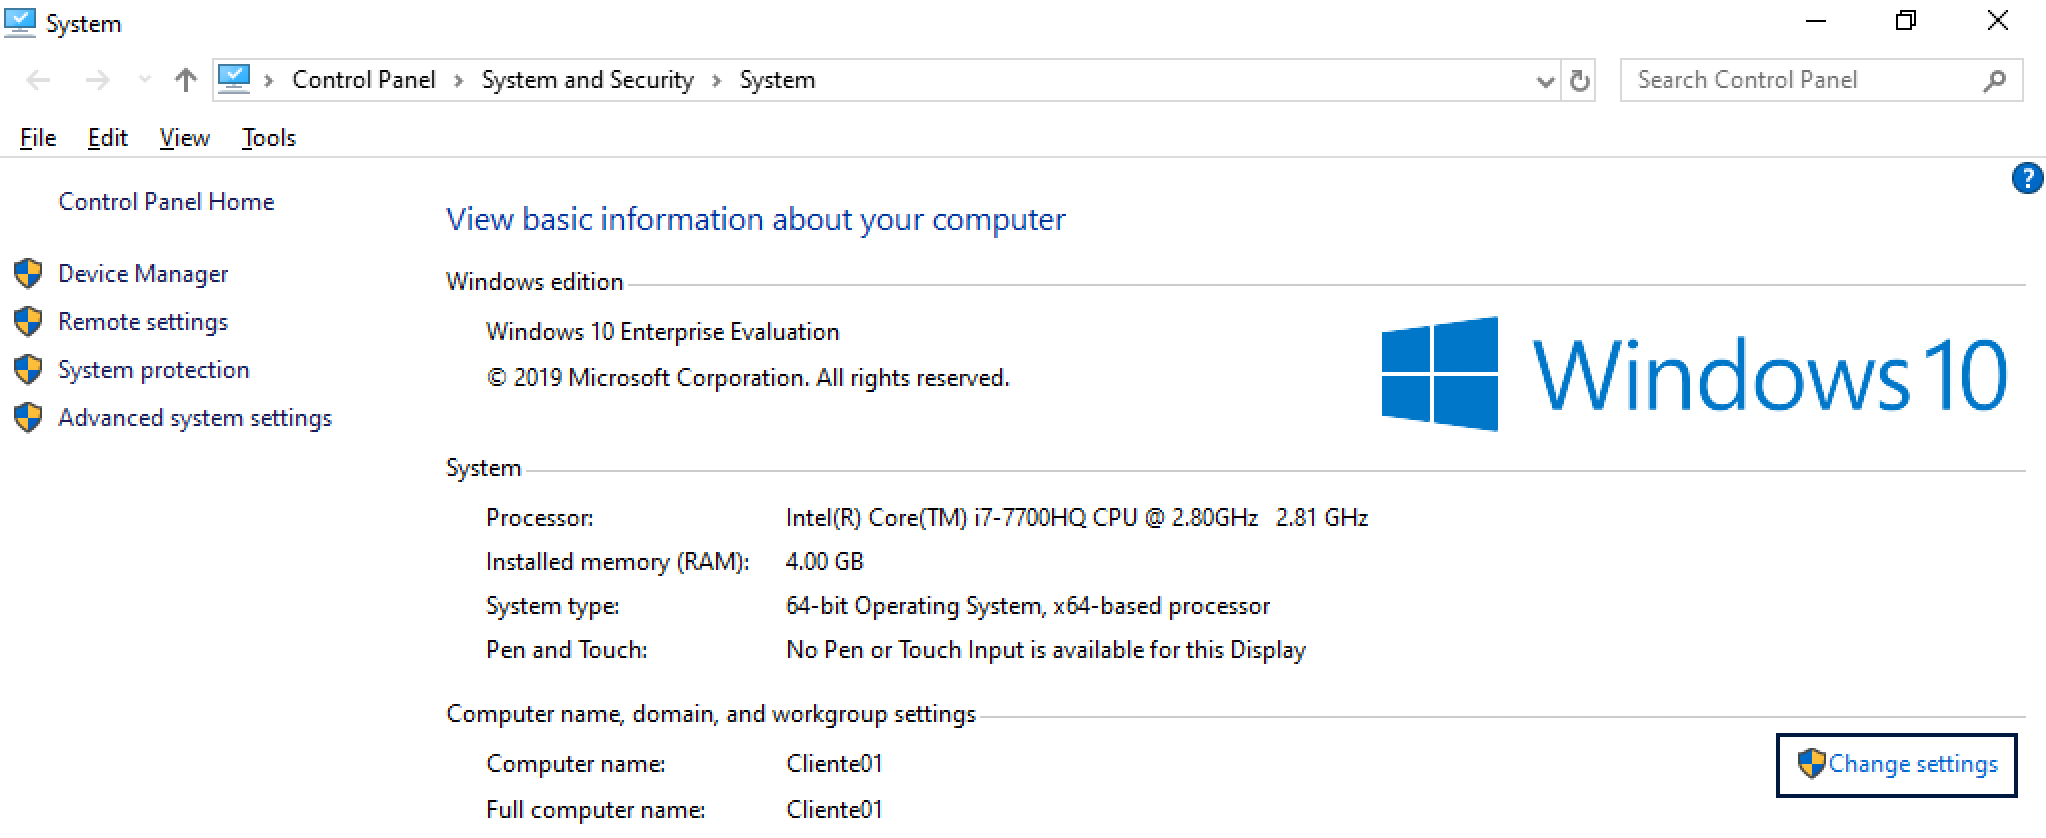
\includegraphics[width=15cm]{DC01/AD1.png}
\end{center}
\caption{Cambio de nombre Cliente01}
\label{DC01-AD1}
\end{figure}




\subsubsection{Intalación y configuración}
\subsubsection{Creación de usuarios y carpetas compartidas}
